\section{Experimentelles Vorgehen und Ergebnisse}
\subsection{Abhängigkeit der Aktingeschwindigkeit von der Konzentration des ATP}
Bei der Versuchsvorbereitung wurden mit Myosin beschichtete Glasplättchen hergestellt.
Danach wurden Aktinfilamente auf das Myosin gegeben wurden und das im Motility Buffer gelöste ATP 
hinzugefügt.
Mit dem Mikroskop und einer CCD Kamera wurden für verschiedene ATP-Konzentrationen alle
100 ms insgesamt 100 Bilder aufgenommen. Mithilfe des Programms "ImageJ" konnte man die Geschwindigkeit
der Aktinfilamente bestimmen. Dabei wurden die Geschwindigkeit jener Aktinfilamente gemessen, die
sich über die Zeit von 100ms kontinuierlich bewegt haben. Bei höheren Konzentrationen von ATP war die
Geschwindigkeit der Aktinfilamente deutlich höher als bei niedriegen Konzentrationen,
wie durch die Michaelis-Menten Gleichung \ref{equ:michaelis_menten} vorhergesagt.

\begin{equation}
  \nu = \frac{\nu_{max} \cdot [S]}{K_m + [S]}
  \label{equ:michaelis_menten}
\end{equation}
Jedoch zeigt der letzte Messpunkt bei der ATP Stoffmenge von 2000$\mu \text{Mol}$ eine starke
Abweichung vom geplottetem Graphen \ref{fig:normal_speed}.
Bereits bei der Versuchdurchführung war die geringe Geschwindigkeit der Filamente aufgefallen.
Diese Abweichung könnte auf einem nicht linearen Zusammenhang zwischen
Aktingeschwindikeit und Produktionsrate des ADP deuten.
Eine weiter Ursache für die niedrigen Geschwindigkeiten könnte ein Pippetierfehler sein,
der der dafür gesorgt hat, dass es eine andere ATP Konzentration in der Lösung gab. 
Um die nichtlinearität genauer zu untersuchen müsste man den Versuch erneut durchführen,
mit mehr Abstufungen verschiedener Konzentrationen.
Bei der Wiederholung des Versuchs müsste man ebenso darauf achten genau zu pippetieren.
Wegen der ungenauen Datenlage kann man keinen einzelnen genauen Wert für die maximale
Aktingeschwindikgeit oder die Gleichgewichtskonstante angeben.
Es wurden zwei Fits durchgeführt, dabei wurde einmal der letzte Wert in den Fit mit einbezogen und einmal weggelassen. 
\begin{figure}[]
  \centering
  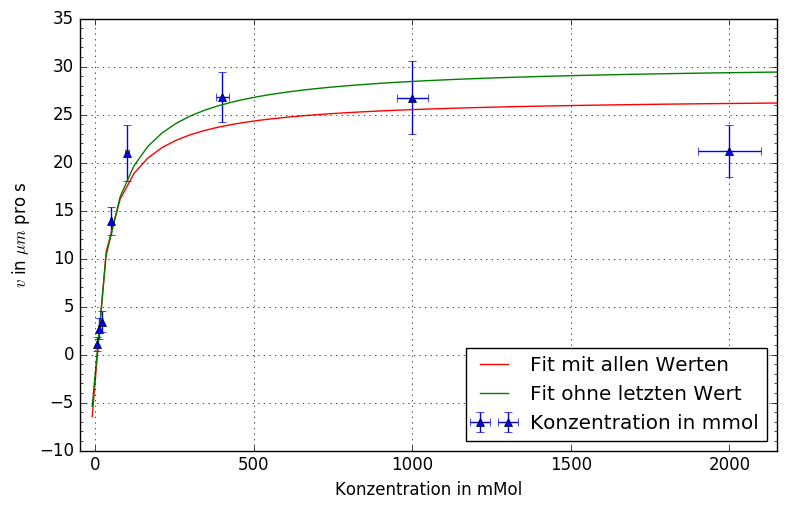
\includegraphics[width=0.8\textwidth]{bilder/both_fits.png}
  \caption{gemessene Aktingeschwindigkeit in $\sfrac{\mu m}{s}$ in A}
  \label{fig:normal_speed}
\end{figure}

\begin{figure}[]
  \centering
  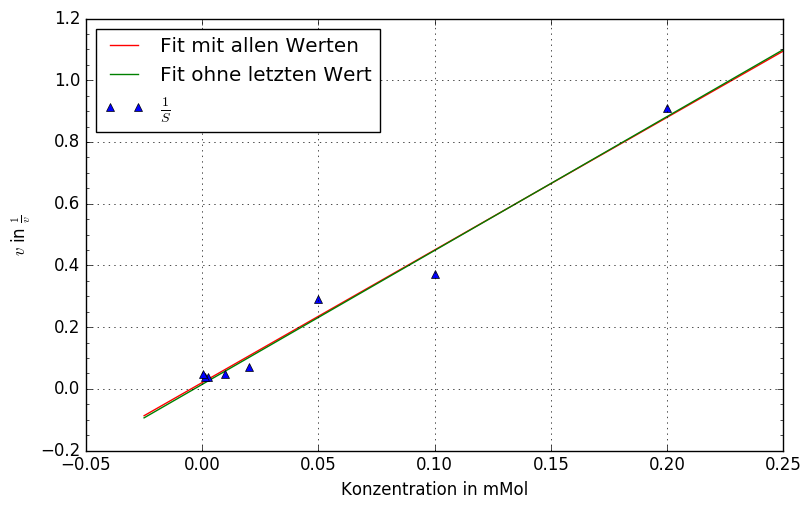
\includegraphics[width=0.8\textwidth]{bilder/both_fits_1over.png}
  \caption{Fit über 1/$\nu$  in $\sfrac{s}{\mu m}$ in A}
  \label{fig:1_over_speed}
\end{figure}

%%% Local Variables:
%%% mode: latex
%%% TeX-master: "../motors"
%%% End:
